\section*{Materiali e metodi}

Si comincia col dare una panoramica generale dei metodi di misura e acquisizione dati tramite impulsi CPMG e IR. Si prosegue poi con la descrizione della strumentazione utilizzata e dei parametri di misura scelti per i campioni di tuorlo e albume.

\subsection*{Metodo CPMG e IR}

Quando si misurano i tempi di rilassamento $T_1$ e $T_2$ si vanno ad acquisire curve sperimentali di rilassamento seguendo l'evoluzione nel tempo del vettore magnetizzazione dopo una perturbazione.

Quello che tuttavia è possibile misurare è solamente la componente del vettore magnetizzazione nel piano trasversale.

Questa componente viene misurata in unità arbitrarie $S(t)$ e, acquisendo coppie di valori $(S(t), t)$, si vanno a costruire le curve di rilassamento, sulle quali viene poi effettuata l'opportuna analisi dati.

\paragraph{Metodo IR.}

Il metodo \textit{Inversion Recovery} serve per misurare il tempo $T_1$ di rilassamento longitudinale. Siccome ogni misura fatta riguarda solo le componenti trasversali del vettore di magnetizzazione, si esegue prima un impulso di inversione di $180^{\circ}$ sul vettore magnetizzazione non perturbato, poi, dopo un tempo $\tau$ variato di volta in volta, si esegue un secondo impulso di inversione di $90^{\circ}$ per traslare la componente $M_z(\tau)$ sul piano $(x,y)$ e misurarne i valori. Per ottenere un impulso di inversione di $180^{\circ}$ si può sia fare uso di un campo magnetico di intensità doppia rispetto a quello usato dall'impulso di $90^{\circ}$; oppure fare uso della stessa intensità, ma con una durata di applicazione doppia (Figura \ref{fig:inversioni}).

\begin{figure}[ht]
\centering
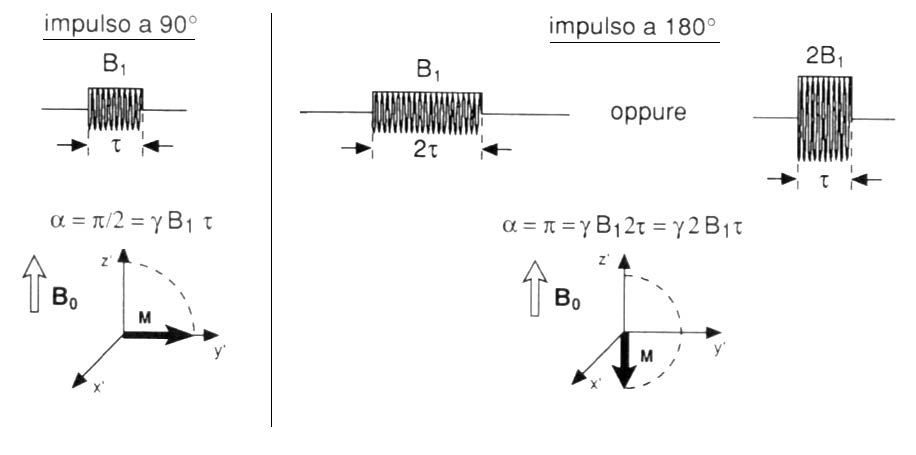
\includegraphics[width=\textwidth]{inversioni.jpg}
\caption{Confronto grafico tra impulso di inversione di $90^{\circ}$ e due varianti di impulso di $180^{\circ}$.}
\label{fig:inversioni}
\end{figure}  

Variando il valore di $\tau$ e misurando il picco del segnale di FID che avviene dopo la seconda inversione, è possibile tracciare la curva del rilassamento longitudinale a partire dalla formula ideale:
\begin{equation}
	M_z(\tau)=M_0\left(1 - 2e^{-\frac{\tau}{T_1}}\right)
\end{equation}
Per contemplare però anche le inevitabili disomogeneità sperimentali del campo $B_1$, si considera un parametro di smorzamento $\eta$ tale che:
\begin{equation}
	M_z(\tau)=M_0\left(1 - (1+\eta)e^{-\frac{\tau}{T_1}}\right)
\end{equation}

Per visualizzare meglio il processo, si rimanda il lettore alla Figura \ref{fig:ir}.

\begin{figure}[ht]
\centering
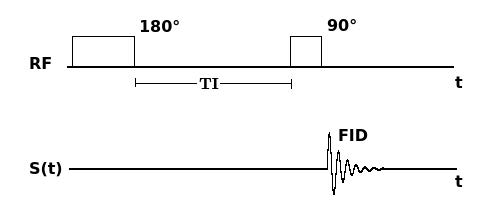
\includegraphics[width=\textwidth]{ir.jpg}
\caption{Segnale ottenuto tramite sequenza di impulsi IR.}
\label{fig:ir}
\end{figure}

\paragraph{Metodo CPMG.}

Il metodo \textit{Carr-Purcell-Meiboom-Gill} viene usato per ottenere una misura di $T_2$ priva dei bias causati dalla non uniformità del campo magnetico applicato $B_0$ e dagli effetti di diffusione molecolare interni al campione.

Queste imperfezioni, infatti, fanno sì che con una misura tramite FID venga sempre misurato un tempo di rilassamento $T_2^*$ molto minore del $T_2$ "vero", causato solo dalle interazioni intrinseche del sistema. Inoltre, il metodo CPMG risulta più efficace rispetto al metodo Spin Echo (SE) in quanto riduce consistentemente gli effetti di diffusione molecolare, causati sempre dal gradiente del campo magnetico $B_0$.

Il metodo CPMG può essere presentato come un ampliamento del metodo SE: ottenuto un segnale di NMR con un segnale di impulso di $90^\circ$, si vogliono rimuovere gli effetti di decadimento causati dalla inomogeneità di $B_0$ applicando segnali di inversione di $180^\circ$. Tuttavia, invece di applicare un solo segnale di inversione a diversi tempi $\tau_i$ per poi misurare le conseguenti ampiezze di segnale di eco di spin, si va ad applicare una sequenza di segnali di inversione $(\tau_0 - 180^\circ - \tau_0)_n$ dove $\tau_0$ è il tempo più breve possibile ottenibile a livello strumentale.\\

Riassumendo, con un metodo di acquisizione tramite FID si misura un tempo di decadimento $T_2^*$, che in letteratura viene spesso assunto nella forma:
\begin{equation}
	\frac{1}{T_2^*} = \frac{1}{T_2} +\frac{1}{T_2'}
\end{equation}
dove $T_2'$ è la componente di tempo causata dalle imperfezioni del campo $B_0$.

Con il metodo SE, si riesce ad isolare meglio $T_2$. Tuttavia, rimangono gli effetti di diffusione molecolare che inevitabilmente interferiscono ancora con la misura. Indicando con $\tau$ il tempo di attesa prima del segnale di inversione, con $A(2\tau)$ l'ampiezza dell'eco al tempo $2\tau$ e con $A(0)$ il primo segnale NMR rilevato, si ha che:
\begin{equation}
	A(2\tau) = A(0)\exp\left(-\left(\frac{2\tau}{T_2}\right) - \frac{2}{3} \gamma^2 g^2 D \tau^3\right)
\end{equation}
dove $\gamma$ è il rapporto giromagnetico, $g$ è l'intensità del gradiente e $D$ è il coefficiente di diffusione.

Con il metodo CPMG, invece, si riescono a confinare gli effetti di diffusione. 
Essendo $\tau_0$ costante ed avendo molteplici segnali di eco di spin, si ha che:
\begin{equation}
	A(t) = A(0)\exp\left(-\left(\frac{t}{T_2}\right) - \frac{1}{3} \gamma^2 g^2 D \tau^2\right)
\end{equation}

Per visualizzare meglio il processo CPMG, si rimanda il lettore alla Figura \ref{fig:cpmg}.

\begin{figure}[ht]
\centering
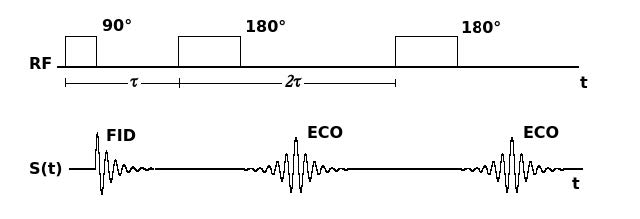
\includegraphics[width=\textwidth]{cpmg.jpg}
\caption{Segnale ottenuto tramite sequenza di impulsi CPMG.}
\label{fig:cpmg}
\end{figure}

\subsection*{Strumenti utilizzati e parametri sperimentali}

Per acquisire le curve di rilassamento longitudinale e trasversale dei campioni di albume e tuorlo, si è fatto uso di un rilassometro costituito da un elettromagnete Jeol, pilotato da una console Stelar per la gestione degli esperimenti NMR e l'acquisizione dati.

Il campo magnetico al quale sono state compiute le misure è $B_0 = 0.473\si{\,}{T}$, corrispondente alla frequenza di Larmor $\nu = 20.15\si{\,}{MHz}$ per il nucleo di idrogeno.

I due campioni sono stati collocati in provette NMR di $8\si{\,}{mm}$ di diametro interno, per una altezza di circa $6\si{\,}{mm}$.

Si riportano tutti i principali parametri di misura in Tabella \ref{tab:setup}.

\begin{table}[ht]
	\centering
	\begin{tabular}{|l|c|c|}
	\toprule
						& \textbf{Tuorlo}& \textbf{Albume}	\\
	\midrule
						& CPMG 			& CPMG 				\\
	\midrule
	Durata impulso $90^{\circ}$ & $3.9\si{\,}{\mu s} $& $3.8\si{\,}{\mu s}$ \\
	TE 					& $200\si{\,}{ms} $	& $200\si{\,}{ms}$ \\
	TR 					& $5\si{\,}{s}$ 	& $5\si{\,}{s}$ \\
	numero echi 		& 32768 		& 32768 \\
	numero scansioni 	& 4 			& 4 \\
	\midrule
	\midrule
						& IR			& IR				\\
	\midrule
	Durata impulso $90^{\circ}$ & $3.9\si{\,}{\mu s} $& $3.8\si{\,}{\mu s}$ \\
	TR 					& $10\si{\,}{s}$	& $10\si{\,}{s}$ \\
	TI iniziale 	 	&$100\si{\,}{\mu s}$& $1000\si{\,}{\mu s}$ \\
	TI finale 		 	& $10\si{\,}{s}$	& $10\si{\,}{s}$ \\
	numero TI in scala LOG & 64			& 64 \\
	numero di scansioni & 1				& 1 \\
	\bottomrule
	\end{tabular}
	\caption{Parametri di misura per i campioni di tuorlo e albume.}
	\label{tab:setup}
\end{table}


\subsection*{Calibrazione}

Per calibrare la sonda collegata al circuito L-C-R, si è eseguito un processo di \textit{tuning} e \textit{matching} della strumentazione tramite utilizzo di un generatore a frequenza variabile.

Nella fase di tuning, si è sintonizzata la frequenza di risonanza con la frequenza di Larmor scelta, modificando la capacità del condensatore in serie in modo da far coincidere il minimo della curva rappresentata dalla console Stelar con la frequenza di Larmor di interesse.

Nella fase di matching, si è fatta coincidere l'impedenza del circuito con la linea di trasmissione a $50\si{\,}{\Omega}$, agendo sul condensatore posto in parallelo alla bobina, in modo da minimizzare il valore del minimo della curva rappresentata dalla console.

Queste procedure sono necessarie per poter gestire gli effetti causati dai materiali diversi presenti all'interno del circuito e massimizzare il rapporto segnale/rumore.

\subsection*{Analisi dati tramite software UPENWin}

Il segnale acquisito è una curva multi-esponenziale nella forma:
\begin{equation}
	S(t) = \sum_{k=0}^M a_k \exp(-t/T_{1/2_k})
\end{equation}
dove si indica con $k$ una delle tante componenti del materiale non uniforme che presenta inevitabilmente tempi di rilassamento $T_1$ e $T_2$ differenti.

Tramite algoritmo UPEN (\textit{Uniform PENality}), implementato nel software UPENWin, si reinterpreta il segnale come una distribuzione continua dei tempi di rilassamento in forma integrale:
\begin{equation}
	S(t) = \int f(T_{1/2}) \exp(-t/T{1/2}) \, dT_{1/2}
\end{equation}
dove $f(T_{1/2})$ è una funzione di distribuzione dei tempi di rilassamento. Per invertire quindi il segnale acquisito ed ottenere una espressione valida della funzione di distribuzione, essendo possibili infinite soluzioni a causa degli errori sperimentali associati ad ogni dato acquisito, il software UPEN fornisce una stima di soluzione in base ad un principio di penalizzazione di soluzioni con eccessivi picchi distinti e non sufficientemente giustificati dai dati.